\documentclass[10pt,twocolumn,letterpaper]{article}

\usepackage{cvpr}
\usepackage{times}
\usepackage{epsfig}
\usepackage{graphicx}
\usepackage{amsmath}
\usepackage{amssymb}

% Include other packages here, before hyperref.

% If you comment hyperref and then uncomment it, you should delete
% egpaper.aux before re-running latex.  (Or just hit 'q' on the first latex
% run, let it finish, and you should be clear).
\usepackage[pagebackref=true,breaklinks=true,letterpaper=true,colorlinks,bookmarks=false]{hyperref}

\cvprfinalcopy % *** Uncomment this line for the final submission

\def\cvprPaperID{****} % *** Enter the CVPR Paper ID here
\def\httilde{\mbox{\tt\raisebox{-.5ex}{\symbol{126}}}}

% Pages are numbered in submission mode, and unnumbered in camera-ready
\ifcvprfinal\pagestyle{empty}\fi
\begin{document}

%%%%%%%%% TITLE
\title{Task 1 \& Task 2: Determining Directions and Reading DICOMs}

\author{Konstantinos Katergaris\\
Arizona State University\\
1151 S Forest Ave, Tempe, AZ\\
{\tt\small kkaterga@asu.edu}}

%\thispagestyle{empty}

\maketitle

\section{Task 1}

\subsection{Introduction}
In this section, the task was to open and write JPG, PNG, and DICOM files from the dataset [1]. When opening JPG and PNG files, only image data was expected, while DICOM files where thought to contain both the image and associated metadata. Additionally, it was hypothesised that all file types could be saved after processing, with the DICOM files preserving the unchanged metadata.

\subsection{Experiments}
The PNG and JPG files were opened using the Python library Pillow \cite{PydicomDocumentation}, and the DICOM file was opened using the library pydicom \cite{PecoDICOM}. After opening the DICOM file, its metadata was printed, and the image was extracted by accessing the pixel array. This pixel array was then converted into an image using Pillow \cite{PillowFromArray}. All images were resized to 64x64 using the resize function \cite{PillowResize} in Pillow, and the PNG and JPG files were saved using the Pillow save function \cite{PillowSave}. For the DICOM image, after resizing, the image was converted back into an array using numpy \cite{NumpyArray}, and the pixel data in the DICOM file was updated with this resized image array. Additionally, the column and row data for the image in the DICOM file were updated. A PNG version of the resized DICOM image was also saved, which required conversion to an 8-bit color range for viewing.

\subsection{{Results}
Figure~\ref{fig} presents the exports of the processing and saving experiments:

\begin{figure}[h!] \centering 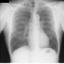
\includegraphics[width=0.2\linewidth]{JPCLN001_resized.jpg} \caption{The resized JPG image} \label{fig
} \end{figure} \begin{figure}[h!] \centering 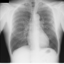
\includegraphics[width=0.2\linewidth]{JPCLN001_resized.png} \caption{The resized PNG image} \label{fig
} \end{figure} \begin{figure}[h!] \centering 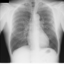
\includegraphics[width=0.2\linewidth]{DICOM.png} \caption{The resized DICOM image } \label{fig
} \end{figure}


\subsection{Conclusion}
The image data was successfully processed and saved without affecting the other metadata in the DICOM file, as initially expected. This is particularly beneficial for using the metadata alongside the image data in a model. Furthermore, the PNG and JPG files were processed and saved as anticipated.
\subsection{Introduction}
The task was to develop a model capable of determining the orientation of chest X-ray images. Initially, the classification head of a pre-trained model was fine-tuned, achieving an accuracy of 0.925, which was considered low for such a straightforward task. This paper investigates training earlier layers of a SWIN Transformer, which ultimately resulted in a perfect accuracy of 1.00.

\subsection{Dataset}
The dataset used \cite{DatasetForClass} consists of chest X-ray images in PNG format with RGB color channels and a resolution of 128x128 pixels. It includes 4 classes: images rotated $0^{\circ}$ (Up), $90^{\circ}$ (Right), $180^{\circ}$ (Down), and $270^{\circ}$ (Left). The dataset contains a total of 988 images, evenly distributed across the 4 classes, with 247 images per class. Of these, 237 images per class are used for training, while the remaining 10 images per class are used for testing. The dataset was loaded into the model using the Huggingface library's dataset object\cite{huggingfacedataset}.

\subsection{Model}
The model developed was a Tiny SWIN-Transformer classifier \cite{DBLP:journals/corr/abs-2103-14030}} from Huggingface Transformers. The classification head was modified to include four output layers, utilizing pre-trained weights \cite{huggingface}.

\subsection{Training}
Image Preprocessing
The images in the dataset were preprocessed using the AutoImageProcess function in the Huggingface Transformers library \cite{huggingfaceproc}, utilizing its pretrained settings \cite{huggingface}. This function automatically handled preprocessing steps such as resizing, along with other procedures employed by the original model.

\subsection{Experiments}
The model was trained using the Huggingface Transformers Trainer\cite{huggingfacetrain}. The optimal base hyperparameters, determined when training only the classifier head, were a learning rate of 5e-4, a batch size of 16, and 10 epochs, resulting in an accuracy of 0.925. To improve these results, earlier layers of the model,specifically the layer before the classifier and two layers before the classifier, were also trained using the same hyperparameters. It was hypothesized that training the layer before the classifier would yield better results without overfitting, while training two layers before would lead to overfitting, reducing the generalizability of the pretrained weights and producing worse training loss and accuracy.

\subsection{Results}
The results for loss convergence in the experiments are shown in Figure~\ref{fig/Loss}, and the accuracy's are presented in Table~\ref{tab:Acc}.

\begin{figure}[h!] 
\centering 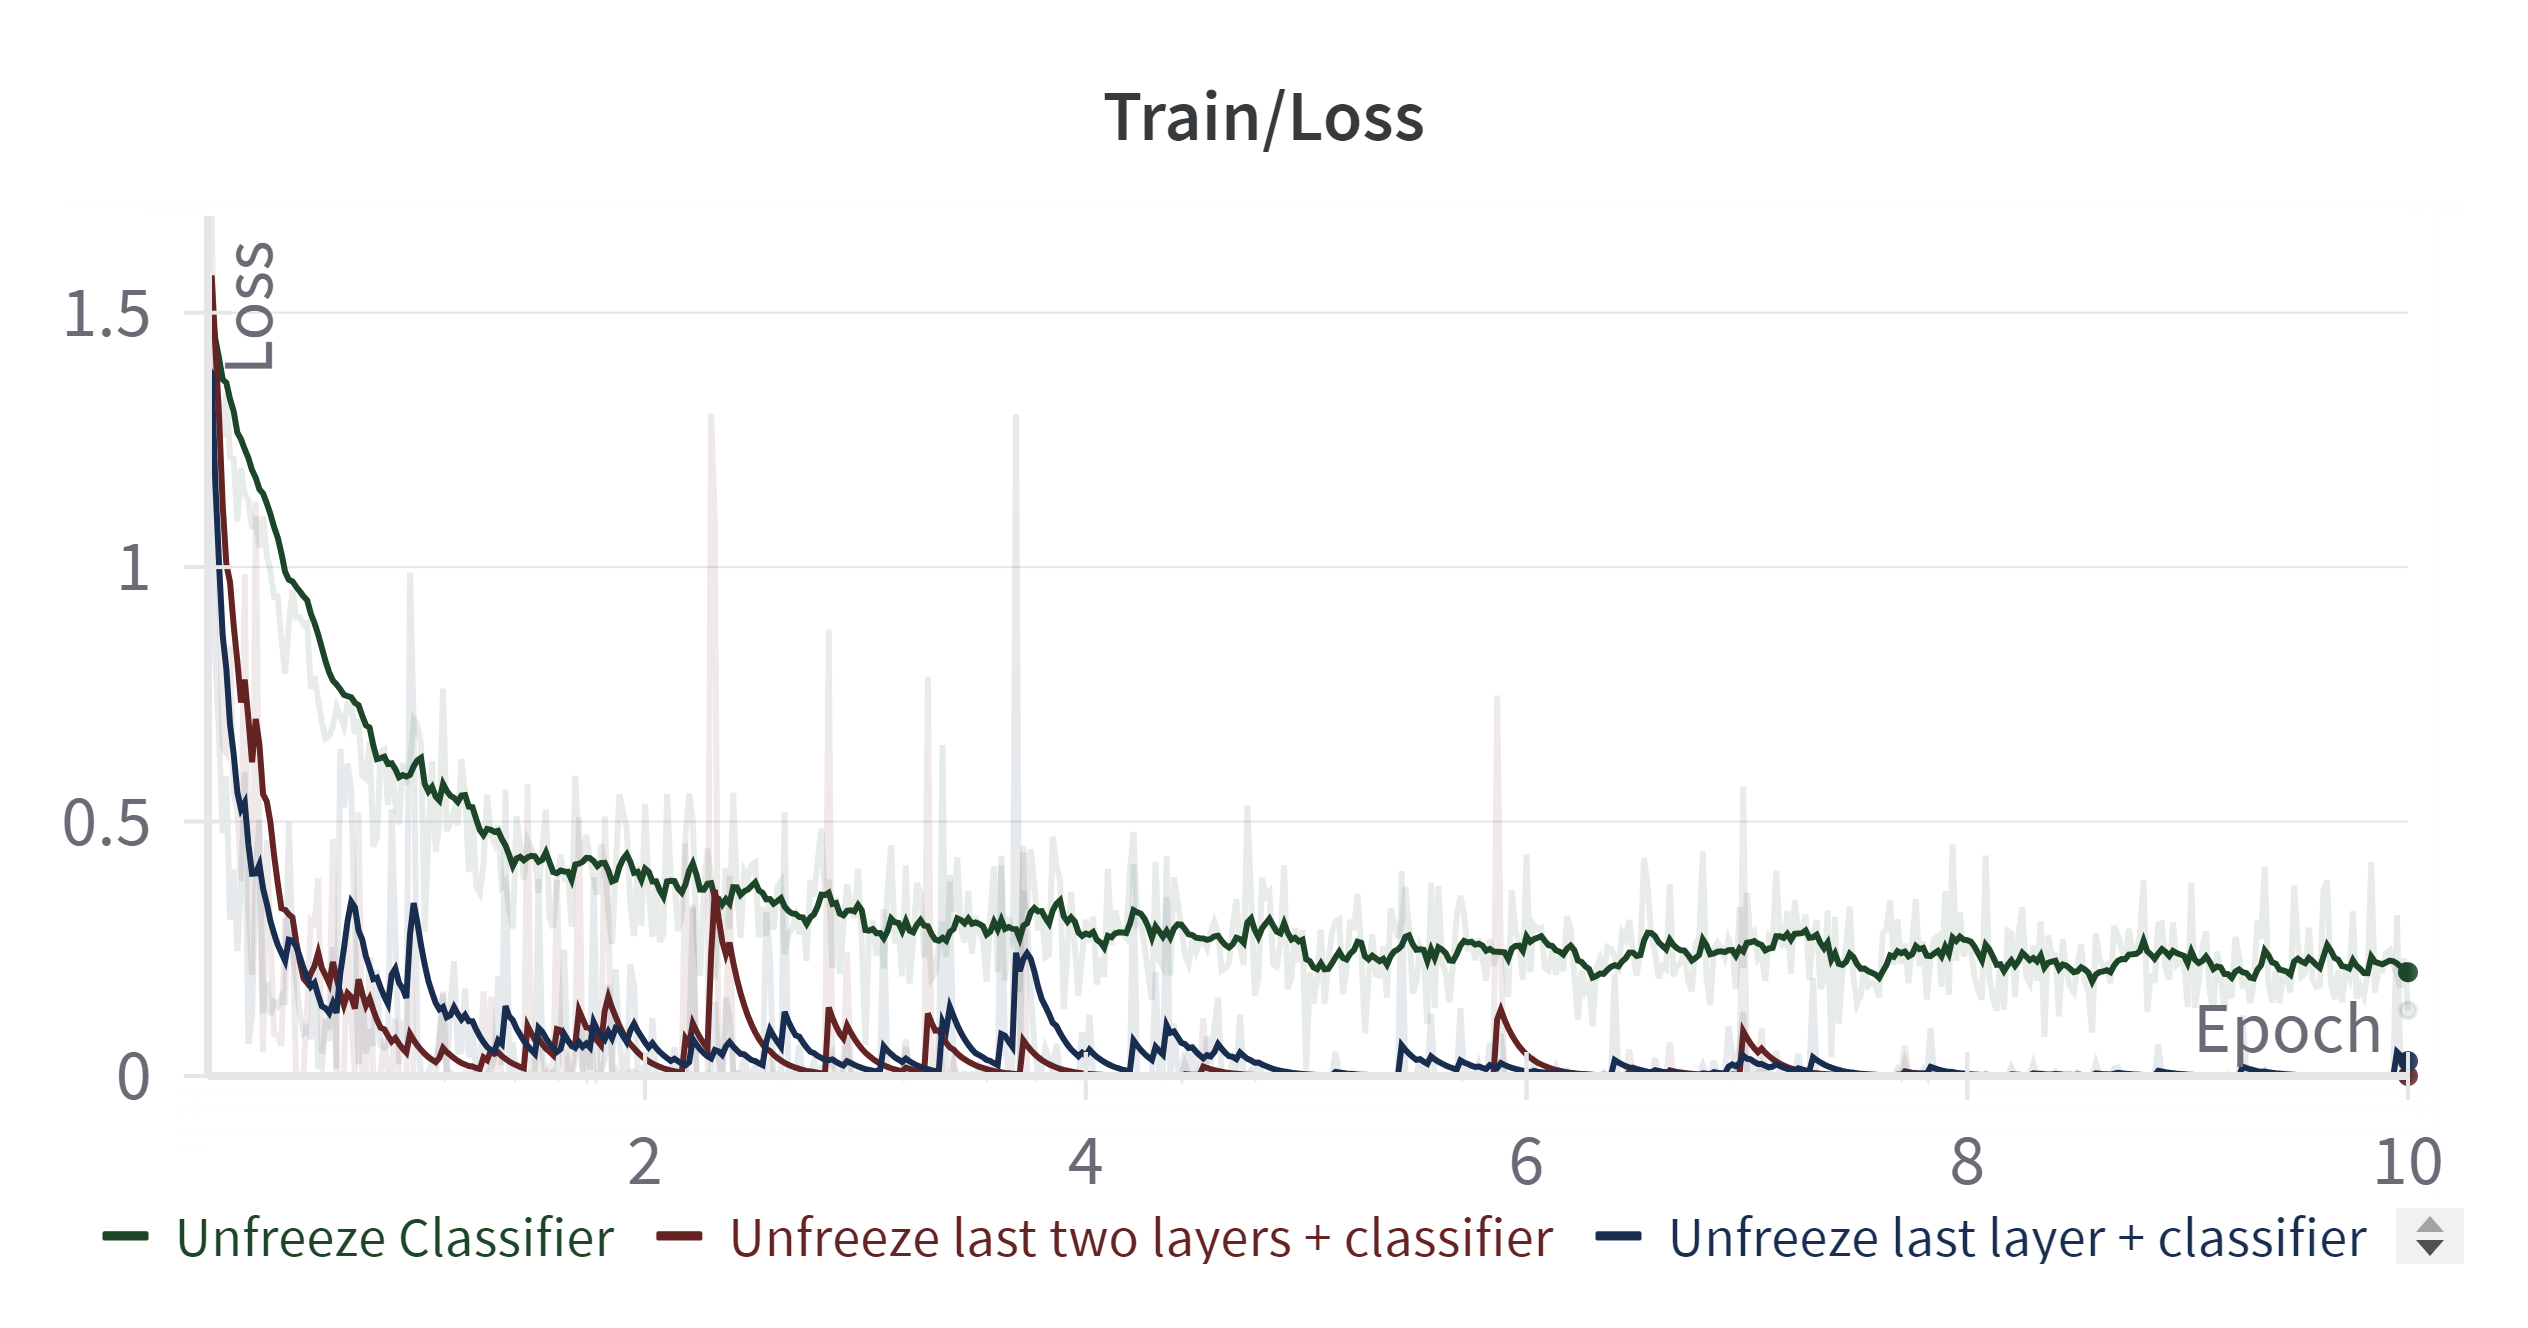
\includegraphics[width=1\linewidth]{Loss Graph (4).png} \caption{ This graph shows the training losses for each experiment. The green line represents the experiment where only the classifier was unfrozen, the red line corresponds to unfreezing the last two layers along with the classifier, and the blue line represents unfreezing the last layer and the classifier. Contrary to the hypothesis, unfreezing the last two layers led to a closer convergence to 0 compared to unfreezing only the last layer. Moreover, it resulted in a lower final loss of 0.0002 versus 0.0291.} 
\label{fig/Loss} 
\end{figure}

\begin{table}[h!]
\begin{center}
\begin{tabular}{|l|c|}
\hline
\textbf{Model} & \textbf{Accuracy} \\
\hline\hline
unfreezing  last layer and  classifier& 1.000 \\
unfreezing  two last layers and  classifier & {1.000} \\
unfreezing classifier & 0.925\\
\hline
\end{tabular}
\end{center}
\caption{This is the overall inference results of the experiments. Unfreezing only the classifier resulted in a 0.925 accuracy. Unfreezing the last two layers along with the classifier and unfreezing the last layer along with the classifier both resulted in an accuracy of 1.000. }
\label{tab:Acc}
\end{table}
\subsection{Conclusion}
Contrary to initial expectations, unfreezing the last two layers along with the classifier performed equally in inference to unfreezing only the last layer and the classifier. However, training deeper layers did lead to better results. It is important to note that overfitting could still be an issue due to the limited test data provided.
{\small
\bibliographystyle{ieee_fullname}
\bibliography{egbib}

}
\end{document}
